\newpage
\begin{center}
\noindent\textbf{ГЛАВА 3. ВЕРХНИЕ ОЦЕНКИ ХРОМАТИЧЕСКИХ ЧИСЕЛ СФЕР}\label{chapters:3}
\vspace{1.5mm}
\end{center}

В этой главе приводятся численные результаты и некоторые теоретические рассуждения, продолжающие построения из первой главы. 
Как и раньше, будем обозначать как $G$ двойственный граф триангуляции для некоторой сферической диаграммы Вороного, 
удовлетворяющей условиям \ref{chapter1:eq:diams}, \ref{chapter1:eq:radiuseq}, $G^2$ -- его квадрат. 
Граф триангуляции для диаграмм Вороного с икосаэдральной симметрией обозначается $T(p,q)$.

\vspace{5pt}
\textbf{3.1 Численные эксперименты}\label{chapters:3.1}
\vspace{5pt}

В ходе численных экспериментов были загружены субоптимальные решения задачи Томсона, 
доступные в \textit{Cambridge Cluster Database}. 
Для них (с помощью \textit{QHull}) были построены диаграммы Вороного, двойственные графы триангуляции и их квадраты.  
Задачи о раскраске последних в $7,8,9,10$ цветов были перекодированы в задачи булевой выполнимости (в соответствии с 
формулой \ref{chapter1:eq:formula}), которые подавались на вход нескольким \textit{SAT}-решателям. 
Из полученных раскрасок квадратов двойственных графов были восстановлены раскраски сферы, вычислены диапазоны радиусов, 
при которых эти раскраски корректны (выполнены условия \ref{chapter1:eq:diams}, \ref{chapter1:eq:radiuseq}). 
Вышеперечисленные шаги были запрограммированы на ЯП Python [Приложение 2,3]. 
Наряду со стандартными функциями языка активно использовались библиотеки \textit{numpy}, \textit{scipy}, \textit{python-sat},  
библиотека для работы с графами \textit{NetworkX}.

Большая часть вычислений выполнялась на сервере с
$14$-ядерным процессором Intel\textsuperscript{\textcopyright} Xeon\textsuperscript{\textcopyright} E5-4660 v3, 
операционной системой Ubuntu. 
Основные результаты вычислений приведены на \figurename{ \ref{chapter3:fig:rad}}, где жирным выделены диапазоны радиусов, 
для которых построены корректные раскраски сферы. Более подробные данные о диапазонах радиусов приведены в Приложении 1.
Отметим, что в тех случаях, когда не удалось раскрасить квадрат двойственного графа в $8$ цветов, 
препятствием стала нехватка вычислительных ресурсов, отсутствие раскраски не было доказано.

\vspace{5pt}
\begin{figure}[h]
\centering
\begin{tikzpicture}[x=3mm,y=1em,thick,scale=1.2]
\draw (0,0) -- (25,0); %9
\draw (0,2) -- (25,2); %8
\draw (0,4) -- (25,4); %7

\draw[dashed] (0,-1) -- (0,5);
\draw[dashed] (25,-1) -- (25,5);

\draw[thickest] (3.06,4) -- (4.335,4);
\draw[thickest] (4.335,2) -- (4.63,2);
\draw[thickest] (4.635,2) -- (6.515,2);
\draw[thickest] (11.06,2) -- (11.675,2);
\draw[thickest] (12.24,2) -- (13.01,2);
\draw[thickest] (15.03,2) -- (15.375,2);
\draw[thickest] (4.63,0) -- (4.635,0);
\draw[thickest] (6.515,0) -- (7.4750000000000005,0);
\draw[thickest] (7.865,0) -- (7.885,0);
\draw[thickest] (8.149999999999999,0) -- (9.81,0);
\draw[thickest] (10.920000000000002,0) -- (11.06,0);
\draw[thickest] (11.675,0) -- (12.24,0);
\draw[thickest] (13.425,0) -- (15.0,0);
\draw[thickest] (15.004999999999999,0) -- (15.03,0);
\draw[thickest] (15.375,0) -- (16.38,0);
\draw[thickest] (16.415,0) -- (22.244999999999997,0);

\node[anchor=west] at (0,-1) {0};
\node[anchor=east] at (25,-1) {5};
\node[anchor=west] at (-10,2) {$\chi(S^2(r)) \leq 8$};
\node[anchor=west] at (-10,0) {$\chi(S^2(r)) \leq 9$};
\node[anchor=west] at (-10,4) {$\chi(S^2(r)) \leq 7$};
\end{tikzpicture}
\caption{Диапазоны радиусов.}
\label{chapter3:fig:rad}
\end{figure}

Отдельно рассматривался случай регулярных конфигураций $T(p,q)$: они были сгенерированы 
методом сечения икосаэдра [Приложение 4]. 
Эти задачи (при $p,q \ge 4$, раскраска в $8$ цветов) оказались достаточно трудоемкими и потребовали порядка 
нескольких часов работы $100$ ядер вычислительного 
кластера ИДСТУ СО РАН, а также применения специализированного \textit{SAT}-решателя \textit{CnC}. 
Автор и научный руководитель благодарят О.С. Заикина за помощь в решении этих задач. Полученные результаты 
сформулированы в следующем утверждении. 

\begin{statement}
\begin{equation}
\begin{split}
\chi(T^{2}(2,2)) = 8; \\
\chi(T^{2}(2,3)) = 8; \\
\chi(T^{2}(2,4)) = 8; \\
\chi(T^{2}(2,5)) = 8; \\
\end{split}
\quad\quad
\begin{split}
\chi(T^{2}(3,4)) = 8; \\
\chi(T^{2}(4,4)) = 8; \\
\chi(T^{2}(5,5)) = 8. \\
\end{split}
\end{equation}
\end{statement}

Аналогично, раскраски для больших $p,q$ не были построены ввиду ограниченности ресурсов. 
Этот результат позволяет выдвинуть следующую гипотезу.

\begin{hypothesis}
Квадраты двойственных графов регулярных (обладающих икосаэдральной симметрией) $(p,q)$-решений задачи Томсона  
являются $8$-хроматическими при $p \ge 2, q \ge 2$.
\end{hypothesis}

На разных этапах экспериментов были установлены и протестированы актуальные на момент составления текста 
версии более $10$ \textit{SAT}-решателей, среди которых
\textit{MapleSat},
\textit{Maple\-COM\-SPS-CHB},
\textit{Maple\-COM\-SPS-LRB},
\textit{Maple\-COM\-SPS-pure-CHB},
\textit{Maple\-COM\-SPS-pure-LRB},
\textit{Sat\-Elite},
\textit{Сadical},
\textit{Crypto\-Mini\-Sat5},
\textit{glu\-co\-se},
\textit{glucose-syrup},
\textit{Kissat},
\textit{Mini\-Sat},
\textit{Picosat},
\textit{lin\-ge\-ling},
\textit{plin\-ge\-ling},
\textit{treen\-ge\-ling},
\textit{RSat},
\textit{CnC}. 
Для компиляции использовался gcc 9.3.0 и опции, указанные авторами. 
В тех случаях, когда это имело смысл, замерялось время. 
В таблицах \ref{chapter3:tab:color10}, \ref{chapter3:tab:color9} 
приведен намеренно соокращенный срез замеров: 
среднее по $10$ запускам (для минимизации случайных эффектов) 
время работы (в секундах) некоторых \textit{SAT}-решателей (с параметрами по умолчанию) 
для различных $N$, раскраска в $10$ и $9$ цветов соответственно.

\begin{table}[h!]
\centering
\captionsetup{justification=centering}
\caption{Сравнение эффективности \textit{SAT}-решателей при раскраске графа в $10$ цветов для различных $N$.} 
\label{chapter3:tab:color10}
\begin{tabular}{@{}|c|c|c|c|c|c|c|c|} 
\Xhline{4\arrayrulewidth}
SAT-решатель          & $192$ & $195$ & $212$ & $282$ & $358$ & $372$ & $400$ \\ \Xhline{4\arrayrulewidth}
lingeling             & 0.197 & 0.161 & 0.196 & 0.194 & 0.238 & 0.26  & 0.266 \\ \hline
Glucose               & 0.054 & 0.054 & 0.055 & 0.075 & 0.095 & 0.095 & 0.105 \\ \hline
MiniSat               & 0.054 & 0.054 & 0.054 & 0.074 & 0.09  & 0.091 & 0.105 \\ \hline
CryptoMiniSat         & 0.025 & 0.024 & 0.026 & 0.034 & 0.035 & 0.037 & 0.039 \\ \hline
Cadical               & 0.032 & 0.034 & 0.037 & 0.038 & 0.035 & 0.042 & 0.051 \\ \hline
MapleCOMSPS-CHB       & 0.061 & 0.044 & 0.049 & 0.071 & 0.075 & 0.08  & 0.097 \\ \hline
MapleCOMSPS-LRB       & 0.053 & 0.044 & 0.045 & 0.066 & 0.075 & 0.077 & 0.083 \\ \Xhline{4\arrayrulewidth}
\end{tabular}
\end{table}

\begin{table}[h!]
\centering
\captionsetup{justification=centering}
\caption{Сравнение эффективности \textit{SAT}-решателей при раскраске графа в $9$ цветов для различных $N$.}
\label{chapter3:tab:color9}
\begin{tabular}{@{}|c|c|c|c|c|c|c|c|}
\Xhline{4\arrayrulewidth}
SAT-решатель          & $192$ & $195$ & $212$ & $282$ & $358$ & $372$ & $400$ \\ \Xhline{4\arrayrulewidth}
lingeling             & 0.237 & 0.262 & 0.338 & 0.35  & 0.385 & 0.258 & 0.287 \\ \hline
Glucose               & 0.088 & 0.075 & 0.064 & 0.056 & 0.094 & 0.136 & 0.207 \\ \hline
MiniSat               & 0.088 & 0.054 & 0.058 & 0.124 & 0.068 & 0.096 & 0.117 \\ \hline
CryptoMiniSat         & 0.059 & 0.024 & 0.024 & 0.137 & 0.054 & 0.272 & 0.063 \\ \hline
Cadical               & 0.095 & 0.034 & 0.115 & 0.105 & 0.348 & 0.355 & 0.125 \\ \hline
MapleCOMSPS-CHB       & 0.072 & 0.052 & 0.077 & 0.081 & 0.111 & 0.167 & 0.098 \\ \hline
MapleCOMSPS-LRB       & 0.065 & 0.044 & 0.064 & 0.075 & 0.097 & 0.156 & 0.095 \\ \Xhline{4\arrayrulewidth}
\end{tabular}
\end{table}

Анализируя эти данные автор пришел к выводу, что сравнение эффективности различных 
реализаций и комбинаций их параметров на формулах такого вида малоинформативно: 
многие из них показывают очень близкие результаты. 
Кое-что можно сказать и о самих задачах. Так, в $10$ и $9$ цветов почти мгновенно покрасились все примеры, 
конфликты встречаются редко, при росте $N$ время работы растет незначительно, что говорит о том, 
что такие задачи оказываются относительно простыми для \textit{SAT}-решателей.
С раскрасками в $8$ цветов ситуация прямо противоположная -- эта задача оказывается 
сложной для \textit{SAT}-решателей и никакие комбинации параметров не позволяют решать ее за разумное время. 
При этом удаление одной вершины степени $5$ снова делает ее простой. 
Представляется, что проблема возникает в момент \enquote{замыкания} раскраски в окрестности одной из таких вершин, 
решатель сталкивается с неразрешимым конфликтом и возвращается глубоко назад по дереву рекурсии.

Для визуализации построенных графов и раскрасок на языке C\texttt{++} разработана программа, 
основанная на графической библиотеке \textit{OpenGL} [Приложениe 5]. 
На \figurename{ \ref{chapter3:fig:viz}} приведены результаты работы программы для раскраски сферы в $9$ цветов, $N=192$.

\FloatBarrier
\begin{figure}[!h]
\centering
\captionsetup{justification=centering}
\begin{minipage}[b]{0.5\linewidth}
\center{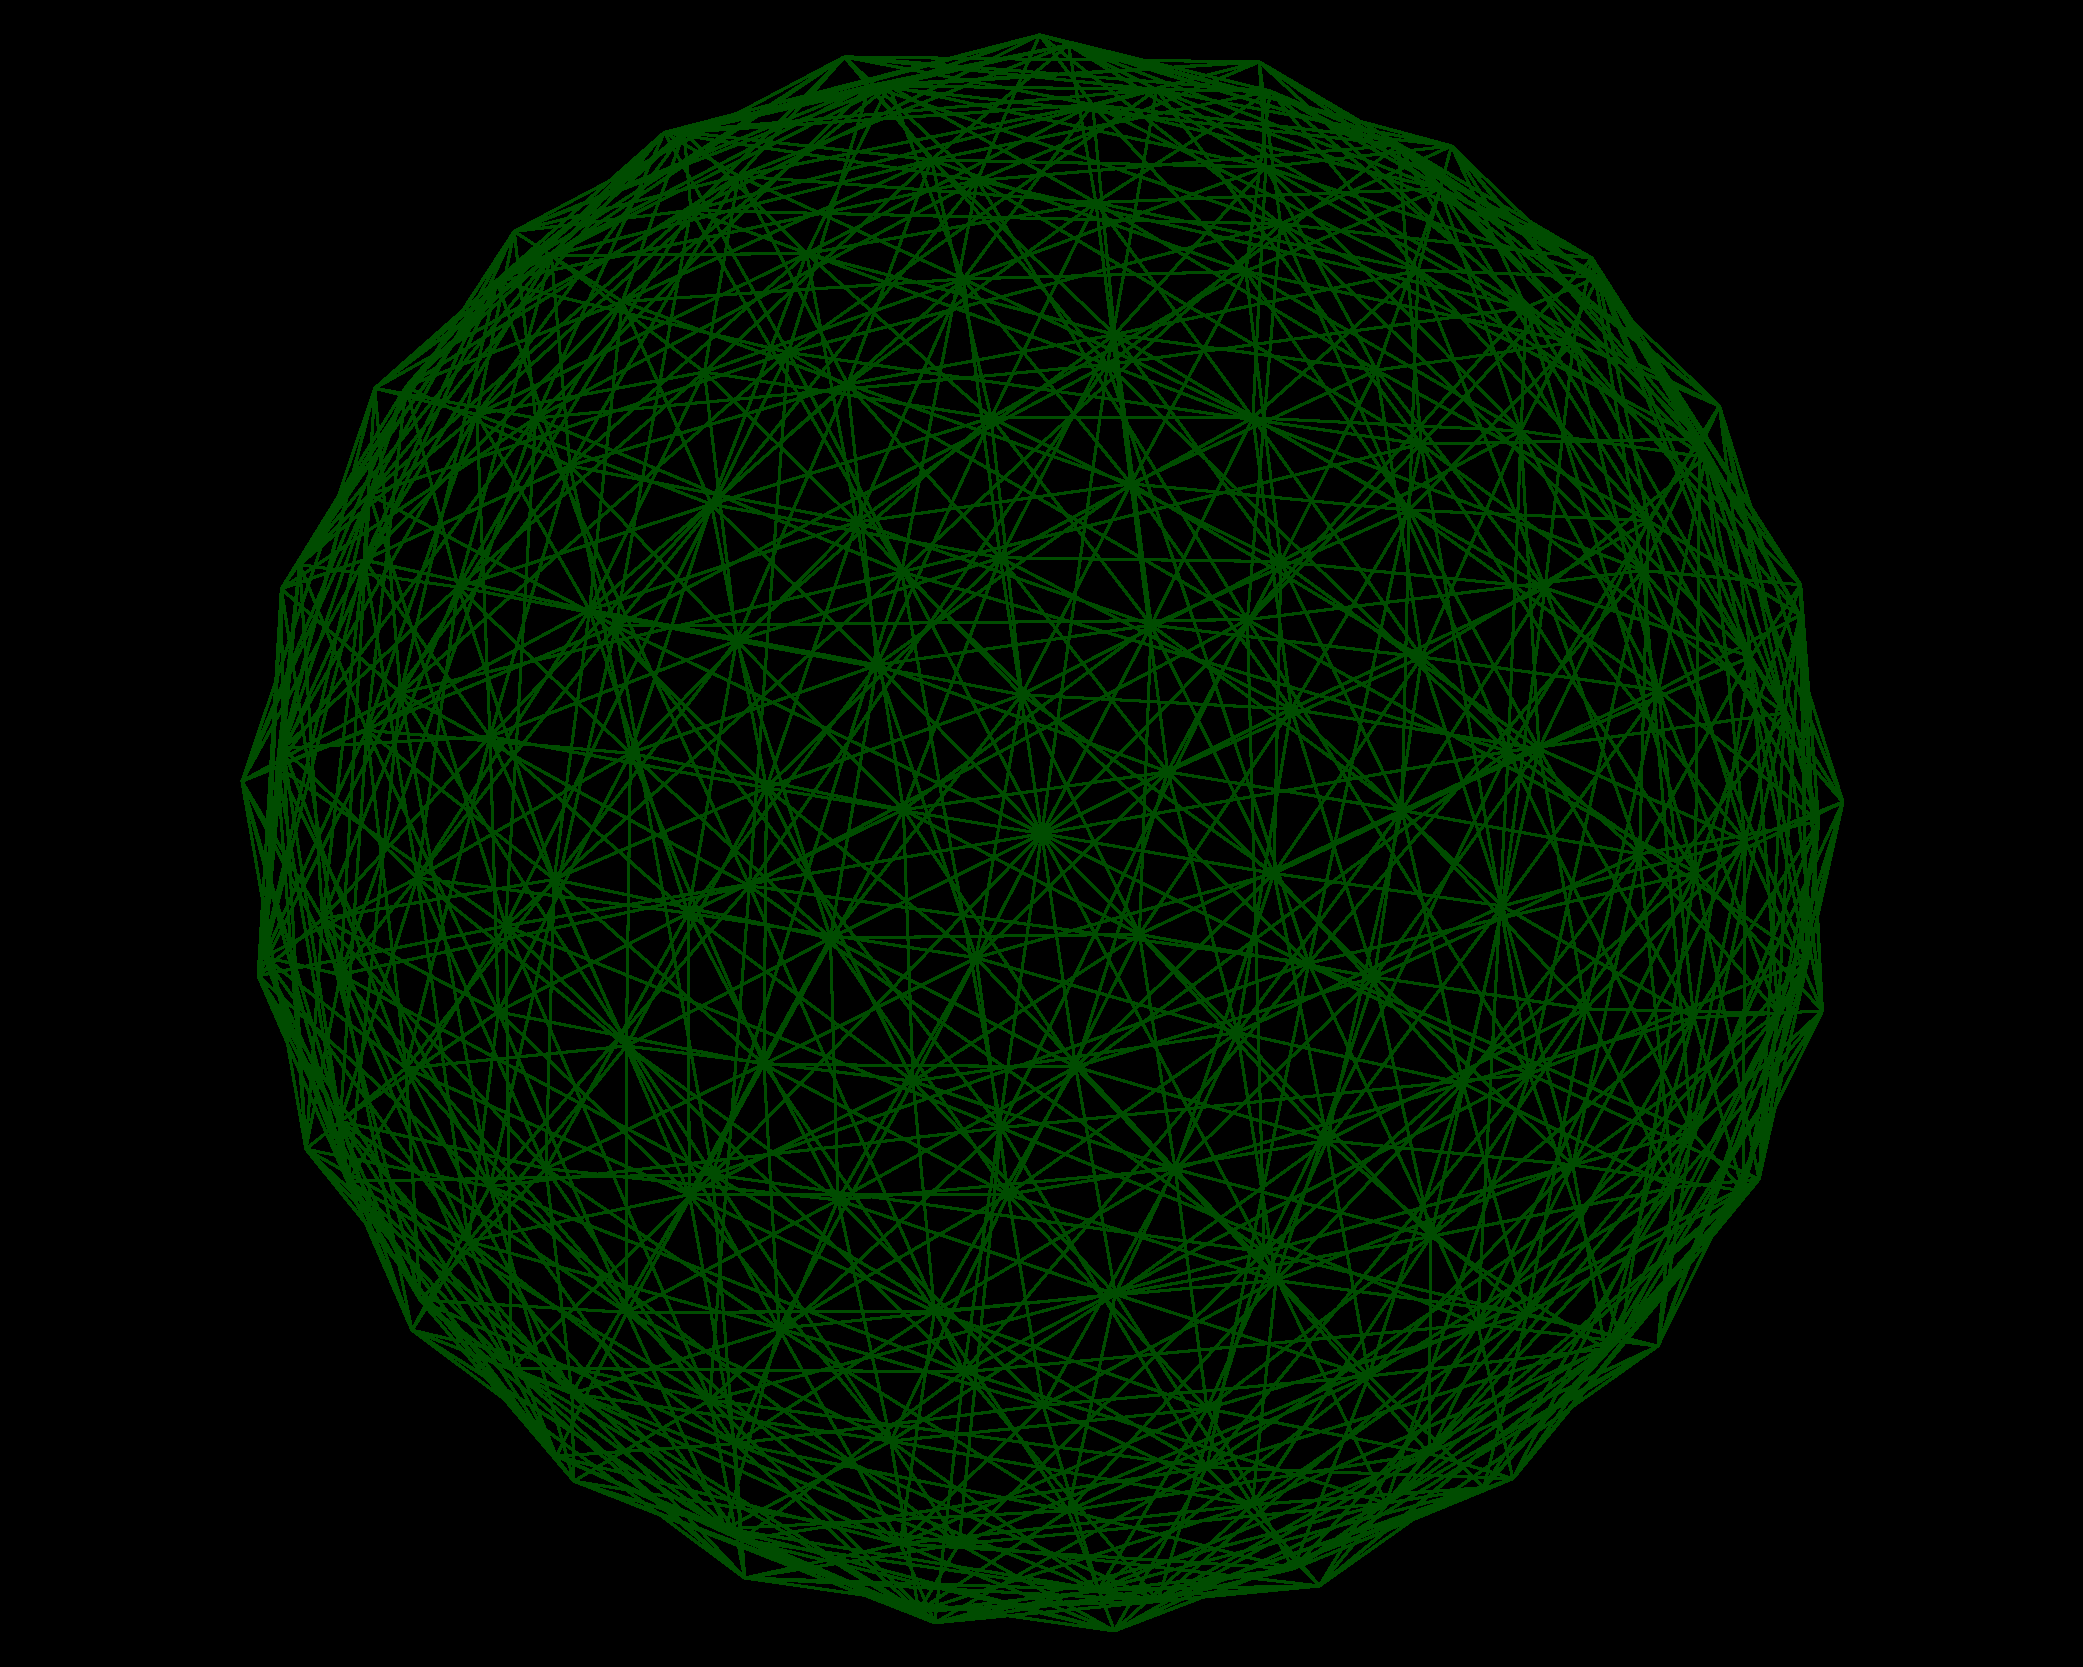
\includegraphics[width=0.37\paperwidth]{chapters/chapter3/program_viz4.pdf}}
\vspace{1ex}
\end{minipage}\hfill
\begin{minipage}[b]{0.5\linewidth}
\center{\includegraphics[width=0.37\paperwidth]{chapters/chapter3/program_viz3.pdf}}
\vspace{1ex}
\end{minipage}\hfill
\begin{minipage}[b]{0.5\linewidth}
\center{\includegraphics[width=0.37\paperwidth]{chapters/chapter3/program_viz2.pdf}}
\vspace{1ex}
\end{minipage}\hfill
\begin{minipage}[b]{0.5\linewidth}
\center{\includegraphics[width=0.37\paperwidth]{chapters/chapter3/program_viz1.pdf}}
\vspace{1ex}
\end{minipage}\hfill
\caption{Пример визуализации раскраски.}
\label{chapter3:fig:viz}
\end{figure}

\vspace{5pt}
\textbf{3.2 Теоретические оценки}\label{chapters:3.2}
\vspace{5pt}

\begin{lemma}\label{chapter3:lemma}
Пусть $G$ содержит такую вершину $v$ степени $5$, что каждая из смежных с ней вершин имеет степень $6$. 
Тогда $\chi(G^2) \ge 8$. В частности, при $p,q \ge 1$ выполнено $\chi(T^2) \ge 8$.
\end{lemma}

\begin{figure}[h]
\centering
\captionsetup{justification=centering}
\center{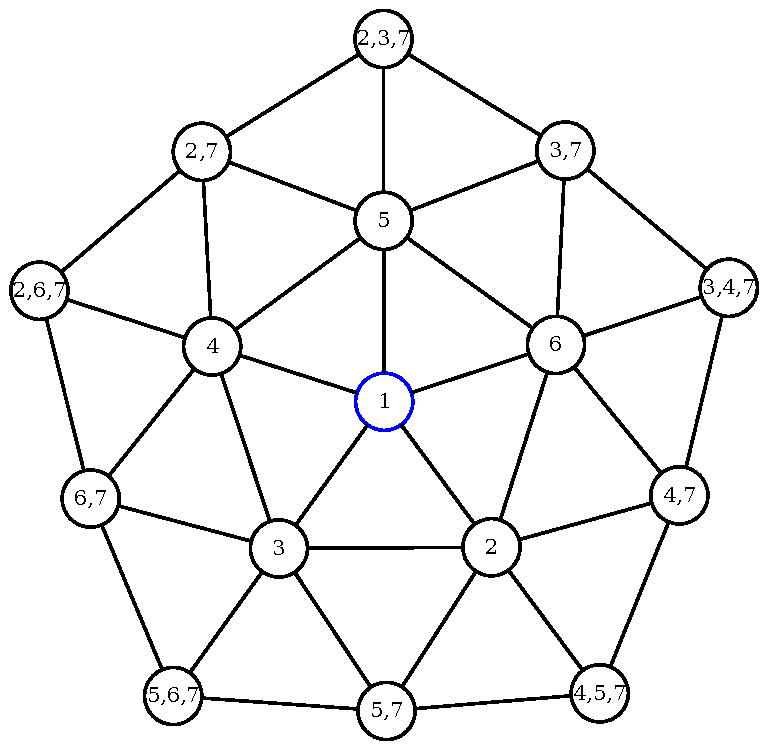
\includegraphics[width=0.45\paperwidth]{chapters/chapter3/cap.pdf}}
\caption{К лемме \ref{chapter3:lemma}.}
\label{chapter3:fig:lemma}
\end{figure}

\begin{proof}
На \figurename{ \ref{chapter3:fig:lemma}} приведены возможные цвета вершин в окрестности вершины степени $5$ (без ограничения общности). 
Тогда из вершин \enquote{внешнего} пояса не более трех имеют цвет $7$, а остальные $7$ вершин раскрашены в цвета $2$--$6$. Но это невозможно, поскольку из этих $7$ вершин можно покрасить в любой из цветов $2$--$6$ не более одной. 
\end{proof}

В заключение приведем набросок доказательства теоремы, 
строгая формулировка которого не была завершена в срок и будет опубликована отдельной статьей.

\begin{theorem}
При некотором $r>r_0$ для раскраски областей сферической диаграммы Вороного,
удовлетворяющей условиям \ref{chapter1:eq:diams}, \ref{chapter1:eq:radiuseq}, 
потребуется по крайней мере $8$ цветов.
\end{theorem}

\begin{myproof}[Идея доказательства.]
0. Предположим, что существует раскраска в $7$ цветов. Тогда нет области с $7$ или более сторонами (для раскраски ее $1$-окрестности потребуется $8$ цветов).

1. Тогда из леммы \ref{chapter3:lemma} следует, что не может быть $5$-угольника, окруженного $6$-угольниками. Верно ли это для вершин двойственного графа степени $3$ и $4$? В любом случае, их не может окружать полоса из $6$-угольников ширины $4$.

2. Рассмотрим подграфы, образованные вершинами степени меньше $6$. Если общий дефект компоненты связности меньше $6$, то вокруг этой компоненты раскраску $6$-угольного замощения невозможно \enquote{склеить} с собой (это возможно только в том случае, если получится цилиндр).

3. Если общий дефект равен $6$, то оценивается максимальный радиус сферы, при которым это возможно (через длину \enquote{пояса} из $6$-угольников).
\end{myproof}